\documentclass[journal]{IEEEtran}
\usepackage[a5paper, margin=10mm, onecolumn]{geometry}
\usepackage{tfrupee}
\usepackage{amsmath, amssymb, amsfonts, amsthm}
\usepackage{algorithmic}
\usepackage{graphicx}
\usepackage{textcomp}
\usepackage{xcolor}
\usepackage{txfonts}
\usepackage{listings}
\usepackage{enumitem}
\usepackage{mathtools}
\usepackage{gensymb}
\usepackage{comment}
\usepackage[breaklinks=true]{hyperref}
\usepackage{tkz-euclide} 
\usepackage{listings}
\usepackage[latin1]{inputenc}                                
\usepackage{color}                                            
\usepackage{array}                                            
\usepackage{longtable}                                       
\usepackage{calc}                                             
\usepackage{multirow}                                         
\usepackage{hhline}                                           
\usepackage{ifthen}                                           
\usepackage{lscape}
\newcommand{\myvec}[1]{\begin{pmatrix} #1 \end{pmatrix}}

\begin{document}

\bibliographystyle{IEEEtran}
\vspace{3cm}

\title{NCERT-11.16.4.3.1}
\author{EE24BTECH11042 - SRUJANA}
{\let\newpage\relax\maketitle}

\renewcommand{\thefigure}{\theenumi}
\renewcommand{\thetable}{\theenumi}
\setlength{\intextsep}{10pt} 

\numberwithin{equation}{enumi}
\numberwithin{figure}{enumi}
\renewcommand{\thetable}{\theenumi}

\textbf{QUESTION}:\\

A die has two faces each with number $'1'$, three faces each with number $'2'$ and one 

face with number $'3'$. If die is rolled once, determine P(2)\\


\textbf{Theoretical solution: }

Total no of possible outcomes = 6 

Favarable outcomes = 3

probability = $\frac{3}{6}$\\

\textbf{Computational Solution:}\\

Let X be a random variable that represents the value of the face when dice is rolled

The PMF of X :

\[
P_X(k) =
\begin{cases}
    \frac{2}{6}, & \text{if } k = 1, \\
    \frac{3}{6}, & \text{if } k = 2, \\
    \frac{1}{6}, & \text{if } k = 3, \\
    0, & \text{otherwise}.
\end{cases}
\]

CDF of X : 
\[
F_X(K) =
\begin{cases}
    0, & x < 1, \\
    \frac{2}{6}, & 1 \leq x < 2, \\
    \frac{5}{6}, & 2 \leq x < 3, \\
    1, & x \geq 3.
\end{cases}
\]
Probability for the face to be 2 is :
$P_X(2) = \frac{3}{6}$\\


\begin{figure}[h!]
   \centering
   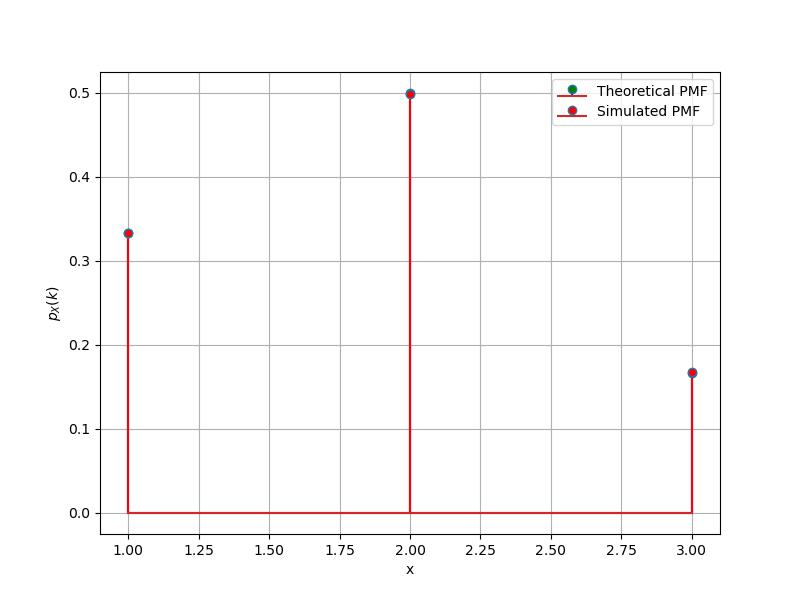
\includegraphics[width=\columnwidth]{figs/pmf.jpg}
   \caption{"PMF Plot"}
\end{figure}


\begin{figure}[h!]
   \centering
   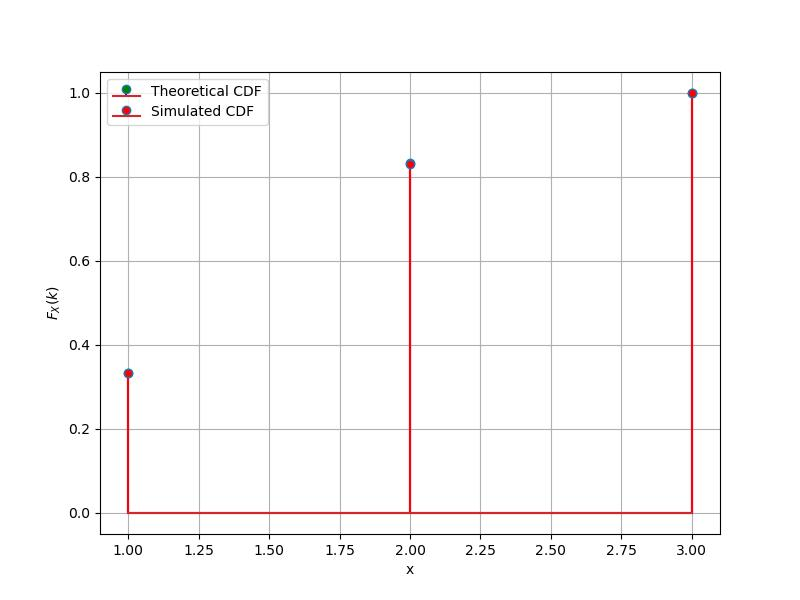
\includegraphics[width=\columnwidth]{figs/cdf.jpg}
   \caption{"CDF Plot"}
\end{figure}



\end{document}
